\documentclass[12pt,letterpaper]{article}
\usepackage[latin1]{inputenc}
\usepackage{amsmath}
\usepackage{amsfonts}
\usepackage{amssymb}
\usepackage{graphicx}

\newtheorem{clm}{Claim}

\author{Linyun Fu}
\title{CSCI 4020 Computer Algorithms Spring 2011\\
Problem Set 4}
\begin{document}
\maketitle
\section*{Chapter 6, Problem 19}
You're consulting for a group of people (who would prefer not to be
mentioned here by name) whose jobs consist of monitoring and analyzing
electronic signals coming from ships in coastal Atlantic waters. They want
a fast algorithm for a basic primitive that arises frequently: ``untangling''
a superposition of two known signals. Specifically, they're picturing a
situation in which each of two ships is emitting a short sequence of 0s
and 1s over and over, and they want to make sure that the signal they're
hearing is simply an \emph{interleaving} of these two emissions, with nothing
extra added in.

This describes the whole problem; we can make it a little more explicit
as follows. Given a string $x$ consisting of 0s and 1s, we write $x^k$ to denote $k$
copies of $x$ concatenated together. We say that a string $x'$ is a repetition
of $x$ if it is a prefix of $x^k$ for some number $k$. So $x' = 10110110110$ is a repetition
of $x = 101$.

We say that a string $s$ is an \emph{interleaving} of $x$ and $y$ if its symbols can be
partitioned into two (not necessarily contiguous) subsequences $s'$ and $s''$,
so that $s'$ is a repetition of $x$ and $s''$ is a repetition of $y$. (So each symbol in
$s$ must belong to exactly one of $s'$ or $s''$.) For example, if $x = 101$ and $y = 00$,
then $s = 100010101$ is an interleaving of $x$ and $y$, since characters 1,2,5,7,8,9
form 101101 -- a repetition of $x$ -- and the remaining characters 3,4,6 form
000 -- a repetition of $y$.

In terms of our application, $x$ and $y$ are the repeating sequences from
the two ships, and $s$ is the signal we're listening to: We want to make sure
$s$ ``unravels'' into simple repetitions of x and y. Give an efficient algorithm
that takes strings $s$, $x$, and $y$ and decides if $s$ is an interleaving of $x$ and $y$.

\section*{Answer}
We use $s[i]$ to denote the $i$-th symbol of $s$, likewise $x[i]$ and $y[i]$. Let $VALID(i,j)$ be the boolean value denoting whether $s[1..i]$ contains a repetition of $x$ with length $j$ and a repetition of $y$ with length $i-j$. We have
\begin{align}
VALID(0,0) = \textrm{true}
\end{align}
and
\begin{align}
\nonumber VALID(i,j) = \textrm{true iff } & \left(s[i] = x[j\hspace{-.7em}\mod |x|]\textrm{ and }VALID(i-1,j-1)\right)\\
& \textrm{ or } \left(s[i] = y[(i-j)\hspace{-.7em}\mod |y|]\textrm{ and }VALID(i-1,j)\right)
\end{align}
for any $i\ge 1, j\ge 1$ and $i\ge j$. Here $|x|$ and $|y|$ denote the length of string $x$ and $y$, respectively, \hspace{-.7em}$\mod$\hspace{-.3em} means the modulo operation, and we let $x[0]=x[|x|]$ and $y[0]=y[|y|]$ to keep it simple. The meaning of Equation~2 is that $s[1..i]$ is an interleaving and contains a repetition of $x$ with length $j$ if and only if its last symbol $s[i]$ belongs to a repetition of $x$ (thus $s[1..i-1]$ contains a repetition of $x$ with length $j-1$) or belongs to a repetition of $y$ (thus $s[1..i-1]$ contains a repetition of $x$ with length $j$).

Based on these equations, and using a two-dimensional array \texttt{VALID[0..n][0..n]} to store the values of $VALID(i,j)$, the algorithm runs as follows.
\\
\tt
VALID[0][0] = true\\
for i from 1 to n do\\
\mbox{\hspace{2em}}for j from 1 to i do\\
\mbox{\hspace{4em}}if s[i] == x[j mod |x|] and VALID[i-1][j-1] then\\
\mbox{\hspace{6em}}VALID[i][j] = true\\
\mbox{\hspace{4em}}else if s[i] == y[(i-j) mod |y|] and VALID[i-1][j] then\\
\mbox{\hspace{6em}}VALID[i][j] = true\\
\mbox{\hspace{4em}}else\\
\mbox{\hspace{6em}}VALID[i][j] = false\\
\mbox{\hspace{4em}}end\\
\mbox{\hspace{2em}}end\\
end\\
\rm

To get the final answer, we check \texttt{VALID[n][0..n]}. If any one of these cells is true, then the answer is true, otherwise the final answer would be false.

The operations performed in the inner loop cost constant time each, and checking \texttt{VALID[n][0..n]} takes time $O(n)$, so the total running time is $O(n^2)$.

\section*{Chapter 6, Problem 28}
Recall the scheduling problem from Section 4.2 in which we sought to
minimize the maximum lateness. There are $n$ jobs, each with a deadline
$d_i$ and a required processing time $t_i$, and all jobs are available to be
scheduled starting at time $s$. For a job $i$ to be done, it needs to be assigned
a period from $s_i \ge s$ to $f_i = s_i + t_i$, and different jobs should be assigned
nonoverlapping intervals. As usual, such an assignment of times will be
called a schedule.

In this problem, we consider the same setup, but want to optimize a
different objective. In particular, we consider the case in which each job
must either be done by its deadline or not at all. We'll say that a subset $J$ of
the jobs is schedulable if there is a schedule for the jobs in $J$ so that each
of them finishes by its deadline. Your problem is to select a schedulable
subset of maximum possible size and give a schedule for this subset that
allows each job to finish by its deadline.
\begin{itemize}
\item[(a)] Prove that there is an optimal solution $J$ (i.e., a schedulable set of
maximum size) in which the jobs in $J$ are scheduled in increasing
order of their deadlines.
\item[(b)] Assume that all deadlines $d_i$ and required times $t_i$ are integers. Give
an algorithm to find an optimal solution. Your algorithm should
run in time polynomial in the number of jobs $n$, and the maximum
deadline $D = max_id_i$.
\end{itemize}

\section*{Answer}

\subsection*{Problem (a)}
First we can assume that the optimal solution is without idle time, because we can simply shift each job after the idle period to an earlier time and every job would still be done by its deadline since it finishes earlier. 

Suppose there exists an inversion in an optimal solution, i.e., job $i$ is scheduled before job $j$ but $d_i > d_j$, then from a previous class of greedy algorithms, we know that there exists two adjacent inverse jobs. We try to prove that swapping such two jobs does not yield a worse schedule.
\begin{figure}
\begin{center}
\includegraphics[width=0.7\textwidth]{4.28.eps}
\caption{Swapping inverse jobs does not make a solution worse}
\end{center}
\end{figure}
Figure~1 shows the effect of swapping such two jobs. Since the finish times of job $i$ and $j$ are both earlier than $d_j$, and the finish times of all the other jobs in the schedule are not affected by the swapping, we know that it is still an optimal solution after the swapping.

So we can start from an arbitrary optimal solution, repeatedly swap adjacent inverse job pairs until there are no more, thus yielding an optimal solution in which jobs are scheduled in increasing order of their deadlines.

\subsection*{Problem (b)}
For the sake of simplicity, we rename all the jobs so that $d_1\le d_2\le...\le d_n=D$, and we subtract the starting time $s$ from every $d_i$ (so now every job can be scheduled from time 0). As we have proven above, there is an optimal solution in which jobs are scheduled in increasing order of their deadlines, so we recognize subproblems as $OPT(i,j)$, which means the maximal number of schedulable jobs among $1, 2, ..., i$ under the constraint that all the chosen job must finish by time $j$. Then $OPT(i,j)$ is achieved either by including job $i$ in the schedule (at the end) or not, i.e.,
\begin{align}
OPT(i,j) = \max{\{OPT(i-1,j-t_i)+1, OPT(i-1,j)\}}
\end{align}
where $i\ge 1$ and $j\ge 0$, and if $j < t_i$, job $i$ cannot be involved in the schedule, so $OPT(i,j) = OPT(i-1,j)$ in this case. And the base case is
\begin{align}
OPT[0][j] = 0 \textrm{ for } j=0, 1, ..., D
\end{align}

Based on these equations, we use a two-dimensional array \texttt{OPT[0..n][0..D]} to store the values of $OPT(i,j)$, and the algorithm runs as follows.
\\
\tt
for j from 0 to D do\\
\mbox{\hspace{2em}}OPT[0][j] = 0\\
end\\
for i from 1 to n do\\
\mbox{\hspace{2em}}for j from 0 to D do\\
\mbox{\hspace{4em}}if j$ < t_i$ then\\
\mbox{\hspace{6em}}OPT[i][j] = OPT[i-1][j]\\
\mbox{\hspace{4em}}else\\
\mbox{\hspace{6em}}OPT[i][j] = max\{OPT[i-1][j-$t_i$]+1, OPT[i-1][j]\}\\
\mbox{\hspace{4em}}end\\
\mbox{\hspace{2em}}end\\
end\\
\rm

The maximal number of schedulable jobs is \texttt{OPT[n][D]}.

To get the optimal solution, we trace back to see how we get to the value \texttt{OPT[n][D]}. We start from \texttt{OPT[n][D]}; at each step, if we see \texttt{OPT[i][j] = OPT[i-1][j]}, we know that job $i$ is not included in the schedule, else if we see \texttt{OPT[i][j] = OPT[i-1][j-$t_i$]+1}, we know that job $i$ is included in the schedule. Doing this backward tracing until we reach \texttt{OPT[0][0]} tells us what jobs are included in the optimal schedule. There may be multiple paths from \texttt{OPT[0][0]} to \texttt{OPT[n][D]}, each of which corresponds to one optimal schedule.

Since sorting all the jobs in increasing order of deadline costs $O(n\log n)$ time, filling out each cell of the array \texttt{OPT[0..n][0..D]} takes constant time, and tracing back to find the actual schedule takes $O(n)$ time, the time complexity of the algorithm is $O(nD)$ (since $\log n = O(D)$ for any reasonable input).

\end{document}
